% Document: Bachelor Thesis: Minimal Problem Solver Generator
% Author: Pavel Trutman

\documentclass[msc]{cmpthesis}
\usepackage{indentfirst}
\usepackage{enumitem}
\usepackage{textcomp}
\usepackage{algorithm}
%\usepackage{algorithmic}
\usepackage{algpseudocode}
\usepackage{amsmath}
\usepackage{amssymb}
\usepackage{forloop}


\usepackage[acronym,nonumberlist,style=long,sort=def]{glossaries}
\setlength{\glsdescwidth}{0.6\linewidth}
\setlength{\glspagelistwidth}{0.4\linewidth}
\renewcommand*{\glsgroupskip}{}
\newcommand{\Acronym}[2]{\newacronym{#1}{#1}{#2}}
\Acronym{C$(f)$, C$(F)$}{Set of all coefficients of the polynomial $f$ or of all polynomials from the set $F$}
\newacronym{deg of f}{$\deg(f)$}{The total degree of $f$}
\newacronym{red}{$\overline{f}^F$}{Remainder of the polynomial $f$ on division by $F$}
\Acronym{gcd}{Greatest common multiple}
\Acronym{lcm}{Least common divisor}
\Acronym{LC$(f)$, LC$(F)$}{Leading coefficient(s) of the polynomial $f$ or of all polynomials from the set $F$}
\Acronym{LM$(f)$, LM$(F)$}{Leading monomial(s) of the polynomial $f$ or of all polynomials from the set $F$}
\Acronym{LT$(f)$, LT$(F)$}{Leading term(s) of the polynomial $f$ or of all polynomials from the set $F$}
\Acronym{M$(f)$, M$(F)$}{Set of all monomials of the polynomial $f$ or of all polynomials from the set $F$}
\Acronym{$S(f_1, f_2)$}{S-polynomial of polynomials $f_1$ and $f_2$}
\Acronym{T$(f)$, T$(F)$}{Set of all terms of the polynomial $f$ or of all polynomials from the set $F$}
\newacronym{x div y}{$x\ |\ y$}{$x$ divides $y$}
\newacronym{floor of x}{$\lfloor x \rfloor$}{$= \max\{m \in \mathbb{Z}\ |\ m \leq x\}$; floor function}
\newacronym{Zp}{$\mathbb{Z}_p$}{Prime field of characteristic $p$}

\makeglossaries


\newcounter{counter}

\renewcommand{\algorithmicrequire}{\textbf{Input:}}
\renewcommand{\algorithmicensure}{\textbf{Output:}}
\algdef{S}[IF]{IfML}[1]{\algorithmicif\ #1}
\newcommand{\StatexIndent}[1][1]{
  \Statex\forloop{counter}{0}{\value{counter} < #1}{\hskip\algorithmicindent\hskip-0.25em}
}

\startThesisInfo
\title{Minimal Problem Solver Generator}
\author{Pavel Trutman}
\CMPAdvisor{Ing. Tom\'a\v s Pajdla, PhD.}
\CMPReportNo{}
\CMPAcknowledgement{\centering Acknowledge grants here. Use centering
   if the text is too short.}

\CMPEmail{pavel.trutman@fel.cvut.cz}
\CMPDocumentURL{http://cmp.felk.cvut.cz/~trutmpav/theses/bsc-pavel-trutman.pdf}
\stopThesisInfo

% ============================== your definitions (abbreviations etc.)
%\def\Ax{\mathbf{A}_x}
\setitemize{noitemsep,topsep=0.2cm,parsep=0.2cm,partopsep=0pt,leftmargin=1cm}

% =========================================================== settings
%\graphicspath{{fig-ch01/}{fig-ch02/}}
\graphicspath{{images/}}

% ========================================================== text body
\begin{document}

\maketitle[3]

\cleardoublepage\def\thepage{\roman{page}}\setcounter{page}{3}
\mbox{}\vfill

{\let\clearpage\relax\par \chapter*{Acknowledgements}}
I would like to thank my advisor Tom\'a\v s Pajdla for introducing me into Gr\"obner basis methods for solving polynomial systems and for his guidance and advices which enabled me to finish this thesis. I would also like to thank Zuzana K\'ukelov\'a for presenting me the automatic generator and for her comments to improvements I have implemented. Special thanks go to my family for all their support.

\clearpage
\chapter*{Abstract}\chapter*{Abstract}
Many problems in computer vision lead to polynomial systems solving. Therefore, we need an easy way how to generate an efficient solver for each problem. On this purpose the automatic generator has been presented. In this thesis we improve the automatic generator so we will be able to generate more efficient and numerically stable solvers.

To improve the automatic generator we review and implement some methods used in the state of the art Gr\"obner basis solvers. Especially, we focus on the $F_4$ Algorithm by Jean-Charles Faug\`ere. Solvers, generated by the automatic generator, can be speed up when efficient methods are used to work with sparse matrices. We describe and implement method which is based on matrix partitioning. This method significantly speeds up the Gauss-Jordan elimination of sparse matrices.

We demonstrate the enhancements of the automatic generator on several important minimal problems. We show that the solvers generated by the new automatic generator are faster and numerically more stable than the solvers generated by the old version of the automatic generator.

\paragraph{Keywords:} computer vision, robotics, minimal problems, polynomials equations, Gr\"ob\-ner basis

\begin{otherlanguage}{czech}
\chapter*{Abstrakt}
Mnoho problémů v počítačovém vidění vede na řešení polynomiálních rovnic. Proto potřebujeme jednoduchý způsob, jak generovat efektivní postupy řešení každého z problémů. Z tohoto důvodu byl představen automatický generátor. V této práci vylepšíme automatický generátor, takže budeme schopni generovat ještě rychlejší a numericky stabilnější postupy řešení polynomiálních systémů.

Abychom mohli vylepšit automatický generátor, prozkoumáme a následně implementujeme některé metody používané v současných nástrojích na řešení soustav polynomiálních rovnic pomocí Gr\"obnerových bází. Zaměříme se zejména na algoritmus $F_4$ představený Jean-Charlesem Faug\`erem. Postupy řešení problémů, vygenerované pomocí automatického generátoru, mohou být ještě dále zrychleny, pokud použijeme efektivní metody na práci s řídkými maticemi. Popíšeme a implementujeme metodu, která je založená na rozkladu matic. Tato metoda výrazně urychluje Gauss-Jordanovu eliminaci řídkých matic.

Vylepšení automatického generátoru předvedeme na několika významných mini\-mál\-ních problémech. Ukážeme, že postupy řešení problémů vygenerované novým automatickým generátorem jsou rychlejší a numericky stabilnější než postupy vygenerované původní verzí automatického generátoru.

\paragraph{Klíčová slova:} počítačové vidění, robotika, minimální problémy, polynomiální rovnice, Gr\"obnerovy báze
\end{otherlanguage}

\clearpage
\chapter*{Resum\'e}Text of resum\'e\dots

\endinput

\cleardoublepage\def\thepage{\arabic{page}}\setcounter{page}{1}
\tableofcontents\pagestyle{headings}
\listofalgorithms

\glsaddall
\printglossary[type=acronym,title=List of Abbreviations]

\chapter{Introduction}
\section{Motivation}
Many problems in computer vision can be formulated using systems of algebraic equations. Examples are the minimal problems \cite{MinimalProblems} which arise when computing geometrical models from image data. The polynomial systems arising from this problems are often not trivial and they consist of many polynomial equations of higher degree in~many unknowns, and therefore general algorithms for solving polynomial systems are not efficient for them. Hence, special solvers for each problem have been developed to solve these system efficiently and robustly.

Minimal problems have a wide range of applications, for example, in 3D reconstruction, recognition, robotics and augmented reality. In these applications, the solvers of~minimal problems are only a small, but very important, part of large computation systems which are supposed be fast or even to work in real-time applications. Moreover, these systems need to compute the solutions of the minimal problems repeatedly for a large number of inputs. Therefore, very efficient solvers are required in computer vision.

Many solvers for minimal problems have been designed ad hoc for concrete problems, and therefore they can not be used or easily modified to solve different or even similar problems. The automatic generator \cite{AutoGen} of minimal problem solvers has been proposed to make this process of the design and generation of the solvers faster and repeatable. This tool generates Gr\"obner basis solvers automatically which enables us to generate an efficient solver for each problem we want to solve.

There are several ways, how the solver using the Gr\"obner basis methods can be generated. The implementation presented in \cite{AutoGen} generates polynomials that are required for solving the system systematically. But other methods can be used, too. In this thesis, we review the state of the art methods for solving polynomials systems and suggest which methods can be taken over to improve the automatic generator and we implement them.

The automatic generator deals with sparse matrices in most cases. Therefore, we may consider to implement some methods which enable us to work with sparse matrices in an~efficient way to save computation time and memory. In this thesis, we focus on how to improve the Gauss-Jordan elimination of sparse matrices. We use the recent work \cite{SBBD} which presents a significant speedup of Gauss-Jordan elimination of sparse matrices. The speed up is caused by transforming matrices into the singly-bordered block-diagonal forms by the paritioning tool PaToH \cite{PaToH}. This method is based on the~fact that more eliminations of smaller matrices are faster than one elimination of a~big matrix.

\section{Thesis structure}
In this thesis, we first review the state of the art methods for computing Gr\"obner basis of polynomial systems. We start with describing simple, but easily understandable, algorithms and continue with more difficult, but also more efficient, algorithms. It is crucial for us to better understand these algorithms because we will use some techniques from them to improve the automatic generator later in this thesis.

Secondly, we briefly describe the automatic generator \cite{AutoGen}. Then, we suggest some improvements of the automatic generator to generate efficient and numerically stable solvers. Some techniques implementened in the automatic generator may be efficient for one minimal problem but may be inefficient for another. Therefore, we present a~benchmark tool which enables us to choose the best methods to generate an efficient solver in the end.

Thirdly, we run some experiments to demonstrate how the implemented improvements have enhanced the automatic generator. We compare the solvers generated by the new automatic generator and the solvers generated by the old implementation.

\section{Notation used}
We have decided to use the notation from \cite{Cox-Little-Shea97} in the whole thesis. We just remind that a polynomial is a sum of terms and a term is a product of a coefficient and a~monomial. Be aware that in some literature, e.g.\ \cite{Becker93, F4, F5}, the meanings of words term and monomial are exchanged.


\chapter{Polynomial system solving}
Firstly we review the state of the art algorithms for computing Gr\"obner basis. Better understanding of these algoritmhs helps us to more efficiently integrate them into polynomial solving algorithms based on Gr\"obner basis computation.

\section{Buchberger's Algorithm}
Buchberger's Algorithm was the first algorithm for computing Gr\"obener basis and it was invented by Bruno Buchberger.

The first and easy, but very inefficient, implementation of this algorithm says that we can extend a set $F$ of polynomials to a Gr\"obner basis only by adding all nonzero remainders $\overline{S(f_i, f_j)}^F$ of all pairs in $F$ into $F$.  The pseudocode of this algorithm can be found as Theorem 2 in Section 2, \S 7 in \cite{Cox-Little-Shea97}. Gr\"obner basis computed by this algorithm are often bigger than necessary.

\section{F4 Algorithm}

\section{F5 Algorithm}


\chapter{Automatic generator}
The automatic generator of Gr\"obner basis solvers is used to easily solve problems leading to systems of polynomial equations. These systems usually arise when solving minimal problems \cite{MinimalProblems} in computer vision. Typically, these systems are not trivial so special solvers have to be designed for concrete problems to achieve efficient and numerically stable solvers. But solvers generated for concrete problems can not be easily applied for similar or new problems and therefore the automatic generator was proposed in \cite{AutoGen}. Solvers generated by the automatic generator can be easily used to solve complex problems even by non-experts users.

The input of the automatic generator is a system of polynomial equations with a finite number of solutions and the output is a MATLAB or a Maple code that computes solutions of the given system for arbitary coefficients. One of the goals of this thesis is to improve previous implementation \cite{AutoGen} of the automatic generator to construct more efficient and numerically stable solvers.

The newest version of the automatic genenerator implemented in MATLAB can be downloaded from \cite{AutomaticGenerator}.

\section{Description of the automatic generator}
In this section we would like to briefly describe the procedure for generating solvers. The automatic generator consists of several independent modules, see Figure \ref{autogen:blockDiagram}. Since all these modules are independent, they can be easily improved or replaced by more efficient implementations. Next we describe each of these modules, full description can be found in \cite{AutoGen}.

\begin{figure}[ht]
  \centering
  \includegraphics[width=0.95\textwidth]{AutomaticGenerator.pdf}
  \caption{Block diagram of the automatic generator}
  \label{autogen:blockDiagram}
\end{figure}

\subsection{Definition of the minimal problem}
Definitions of minimal problems are written in separate functions that are stored in the folder \texttt{minimalProblems}. Each of the definitions has to contain few necessary information about the minimal problem. First of all, the system of polynomial equations with symbolic variables and parameters has to be provided. Next we have to specify the list of unknown variables and known parameters. Optionally if we know the monomial basis $B$ of the polynomial system in advance we can specify it to save some computation time. The monomial basis $B$ is a set $\left\{m\ |\ \overline{m}^G = m\right\}$ where $m$ is a monomial and $G$ is the Gr\"obner basis of the given polynomial system. At last we have to set some settings for the automatic generator. We recommend to obtain the default settings by calling the function \textit{gbs\_InitConfig()} and only overwrite the settings we want to change. In the folder \texttt{minimalProblem} there are some examples which are self explanatory and can be used as templates to create new minimal problem definitions.

\subsection{Equations parser, Instantiating}
In the next step we have to parse the given equations, that means we extract used monomials and parameters and obtain total degrees of the polynomials. Then we instantiate each known parameter with a random number from $\mathbb{Z}_p$. We assign unique identifier to each used parameter. The reason is that we need to track the parameters through the process of adding polynomials in order to be able to restore the process in the solver generation module.

\subsection{Monomial basis $B$ computation}
We need to know the monomials basis $B$ to recognize when we have generated all polynomials that are necessary to build the action matrix. If the basis $B$ was not provided within the definition of the minimal problem we have to compute it by ourselves. Because in MATLAB there is no function or simple script to compute the basis we have to do it by calling an external software.

The most easy solution to implement is to use the Maple toolbox for MATLAB. This enables us to call Maple functions from the MATLAB environment directly. To use this option we have to set \texttt{cfg.GBSolver = @gbs\_findAlgB\_maple} in the settings of the automatic generator. Unfortunately it shows up that the symbolic toolbox provided by Maple in not compatible with the MATLAB symbolic toolbox in versions newer than R2008 so we do not recommend to use this option nowadays, but the option is still available to use on older computers.

The second implemented option is to use the algebraic geometry software Macaulay2 \cite{M2}. In the folder \texttt{gbsMacaulay} there is a template \texttt{code\_template.m2} into which we simply write the given polynomial system. This updated file is saved as \texttt{code.m2} which is executed by Macaulay2 and the results are parsed back in MATLAB. To set up this option we need to install the software Macaulay2 and set \texttt{cfg.GBSolver = @gbs\_findAlgB\_macaulay} in the automatic generator settings. A problem could be that the Macaulay2 is not easy to set up under the Windows OS. Therefore the installation file of Macaulay2 is provided within the automatic generator. The only thing that has to be done is to edit the file \texttt{calc.bat} in the folder \texttt{gbsMacaulay} and follow the instructions in the file.

Because of the modularity of the generator this part can be replaced by another function computing the monomial basis $B$.

The last option is to compute the basis $B$ in advance and set it into the definition of the minimal problem.

In the end we have check the number of solutions of the given polynomial system. If there is a finite number of solutions we can continue with the computation.

\section{Reimplementation}

\section{Multiple eliminations solver}

\section{Removing unnecessary polynomials}

\section{Matrix partitioning}

\section{F4 strategy}


\chapter{Experiments}

\section{Multi elimination solver}
\begin{figure}[ht]
  \centering
  \resizebox{0.9\textwidth}{!}{\input{graphs/elim.tex}}
\end{figure}

\begin{table}[ht]
  \centering
  \begin{tabular}{|c||ccc|}
    \hline
    \textbf{minimal} & 2.159 s & 1.044 s & 1.060 s\\
\textbf{median} & 2.930 s & 2.097 s & 2.015 s\\
\textbf{maximal} & 3.129 s & 2.301 s & 2.444 s\\

    \hline
  \end{tabular}
\end{table}

\section{Matrix partitioning}
\begin{figure}[ht]
  \centering
  \resizebox{0.9\textwidth}{!}{% GNUPLOT: LaTeX picture with Postscript
\begingroup
  \makeatletter
  \providecommand\color[2][]{%
    \GenericError{(gnuplot) \space\space\space\@spaces}{%
      Package color not loaded in conjunction with
      terminal option `colourtext'%
    }{See the gnuplot documentation for explanation.%
    }{Either use 'blacktext' in gnuplot or load the package
      color.sty in LaTeX.}%
    \renewcommand\color[2][]{}%
  }%
  \providecommand\includegraphics[2][]{%
    \GenericError{(gnuplot) \space\space\space\@spaces}{%
      Package graphicx or graphics not loaded%
    }{See the gnuplot documentation for explanation.%
    }{The gnuplot epslatex terminal needs graphicx.sty or graphics.sty.}%
    \renewcommand\includegraphics[2][]{}%
  }%
  \providecommand\rotatebox[2]{#2}%
  \@ifundefined{ifGPcolor}{%
    \newif\ifGPcolor
    \GPcolorfalse
  }{}%
  \@ifundefined{ifGPblacktext}{%
    \newif\ifGPblacktext
    \GPblacktexttrue
  }{}%
  % define a \g@addto@macro without @ in the name:
  \let\gplgaddtomacro\g@addto@macro
  % define empty templates for all commands taking text:
  \gdef\gplbacktext{}%
  \gdef\gplfronttext{}%
  \makeatother
  \ifGPblacktext
    % no textcolor at all
    \def\colorrgb#1{}%
    \def\colorgray#1{}%
  \else
    % gray or color?
    \ifGPcolor
      \def\colorrgb#1{\color[rgb]{#1}}%
      \def\colorgray#1{\color[gray]{#1}}%
      \expandafter\def\csname LTw\endcsname{\color{white}}%
      \expandafter\def\csname LTb\endcsname{\color{black}}%
      \expandafter\def\csname LTa\endcsname{\color{black}}%
      \expandafter\def\csname LT0\endcsname{\color[rgb]{1,0,0}}%
      \expandafter\def\csname LT1\endcsname{\color[rgb]{0,1,0}}%
      \expandafter\def\csname LT2\endcsname{\color[rgb]{0,0,1}}%
      \expandafter\def\csname LT3\endcsname{\color[rgb]{1,0,1}}%
      \expandafter\def\csname LT4\endcsname{\color[rgb]{0,1,1}}%
      \expandafter\def\csname LT5\endcsname{\color[rgb]{1,1,0}}%
      \expandafter\def\csname LT6\endcsname{\color[rgb]{0,0,0}}%
      \expandafter\def\csname LT7\endcsname{\color[rgb]{1,0.3,0}}%
      \expandafter\def\csname LT8\endcsname{\color[rgb]{0.5,0.5,0.5}}%
    \else
      % gray
      \def\colorrgb#1{\color{black}}%
      \def\colorgray#1{\color[gray]{#1}}%
      \expandafter\def\csname LTw\endcsname{\color{white}}%
      \expandafter\def\csname LTb\endcsname{\color{black}}%
      \expandafter\def\csname LTa\endcsname{\color{black}}%
      \expandafter\def\csname LT0\endcsname{\color{black}}%
      \expandafter\def\csname LT1\endcsname{\color{black}}%
      \expandafter\def\csname LT2\endcsname{\color{black}}%
      \expandafter\def\csname LT3\endcsname{\color{black}}%
      \expandafter\def\csname LT4\endcsname{\color{black}}%
      \expandafter\def\csname LT5\endcsname{\color{black}}%
      \expandafter\def\csname LT6\endcsname{\color{black}}%
      \expandafter\def\csname LT7\endcsname{\color{black}}%
      \expandafter\def\csname LT8\endcsname{\color{black}}%
    \fi
  \fi
  \setlength{\unitlength}{0.0500bp}%
  \begin{picture}(8640.00,5040.00)%
    \gplgaddtomacro\gplbacktext{%
      \csname LTb\endcsname%
      \put(946,704){\makebox(0,0)[r]{\strut{} 0}}%
      \csname LTb\endcsname%
      \put(946,1383){\makebox(0,0)[r]{\strut{} 50}}%
      \csname LTb\endcsname%
      \put(946,2061){\makebox(0,0)[r]{\strut{} 100}}%
      \csname LTb\endcsname%
      \put(946,2740){\makebox(0,0)[r]{\strut{} 150}}%
      \csname LTb\endcsname%
      \put(946,3418){\makebox(0,0)[r]{\strut{} 200}}%
      \csname LTb\endcsname%
      \put(946,4097){\makebox(0,0)[r]{\strut{} 250}}%
      \csname LTb\endcsname%
      \put(946,4775){\makebox(0,0)[r]{\strut{} 300}}%
      \csname LTb\endcsname%
      \put(1078,484){\makebox(0,0){\strut{}-15}}%
      \csname LTb\endcsname%
      \put(2511,484){\makebox(0,0){\strut{}-10}}%
      \csname LTb\endcsname%
      \put(3944,484){\makebox(0,0){\strut{}-5}}%
      \csname LTb\endcsname%
      \put(5377,484){\makebox(0,0){\strut{} 0}}%
      \csname LTb\endcsname%
      \put(6810,484){\makebox(0,0){\strut{} 5}}%
      \csname LTb\endcsname%
      \put(8243,484){\makebox(0,0){\strut{} 10}}%
      \put(176,2739){\rotatebox{-270}{\makebox(0,0){\strut{}Frequency}}}%
      \put(4660,154){\makebox(0,0){\strut{}log$_{10}\Big(\big|$error$\big|\Big)$}}%
      \put(4660,4665){\makebox(0,0){\strut{}}}%
    }%
    \gplgaddtomacro\gplfronttext{%
      \csname LTb\endcsname%
      \put(7256,4602){\makebox(0,0)[r]{\strut{}Without matrix partitioning (0 zero errors)}}%
      \csname LTb\endcsname%
      \put(7256,4382){\makebox(0,0)[r]{\strut{}Last elimination with matrix partitioning (0 zero errors)}}%
      \csname LTb\endcsname%
      \put(7256,4162){\makebox(0,0)[r]{\strut{}All eliminations with matrix partitioning (0 zero errors)}}%
    }%
    \gplbacktext
    \put(0,0){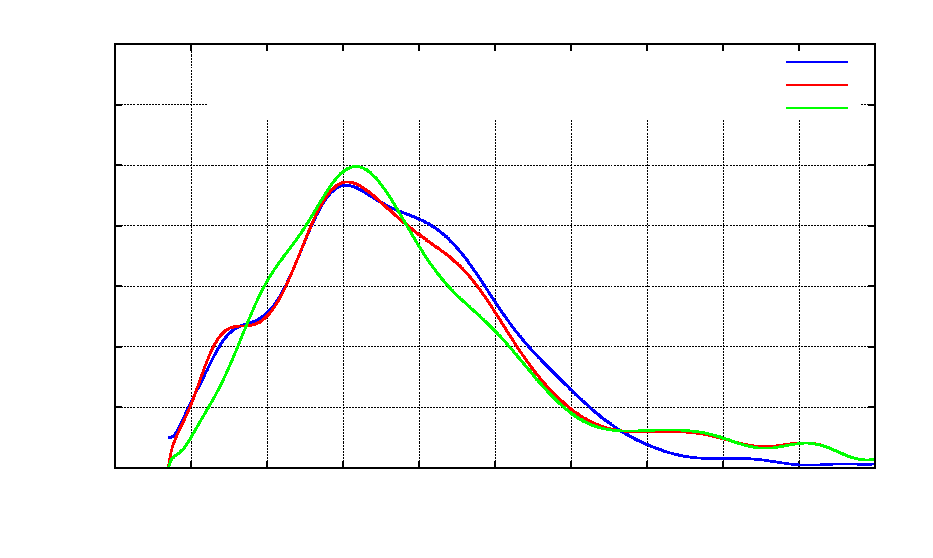
\includegraphics{graphs/part}}%
    \gplfronttext
  \end{picture}%
\endgroup
}
\end{figure}

\begin{table}[ht]
  \centering
  \begin{tabular}{|c||ccc|}
    \hline
    \textbf{minimal} & 1.373 & 1.541 & 0.780\\
\textbf{median} & 2.292 & 2.231 & 0.842\\
\textbf{maximal} & 2.525 & 2.494 & 1.097\\

    \hline
  \end{tabular}
\end{table}

\section{$F_4$ strategy}
\begin{figure}[ht]
  \centering
  \resizebox{0.9\textwidth}{!}{% GNUPLOT: LaTeX picture with Postscript
\begingroup
  \makeatletter
  \providecommand\color[2][]{%
    \GenericError{(gnuplot) \space\space\space\@spaces}{%
      Package color not loaded in conjunction with
      terminal option `colourtext'%
    }{See the gnuplot documentation for explanation.%
    }{Either use 'blacktext' in gnuplot or load the package
      color.sty in LaTeX.}%
    \renewcommand\color[2][]{}%
  }%
  \providecommand\includegraphics[2][]{%
    \GenericError{(gnuplot) \space\space\space\@spaces}{%
      Package graphicx or graphics not loaded%
    }{See the gnuplot documentation for explanation.%
    }{The gnuplot epslatex terminal needs graphicx.sty or graphics.sty.}%
    \renewcommand\includegraphics[2][]{}%
  }%
  \providecommand\rotatebox[2]{#2}%
  \@ifundefined{ifGPcolor}{%
    \newif\ifGPcolor
    \GPcolorfalse
  }{}%
  \@ifundefined{ifGPblacktext}{%
    \newif\ifGPblacktext
    \GPblacktexttrue
  }{}%
  % define a \g@addto@macro without @ in the name:
  \let\gplgaddtomacro\g@addto@macro
  % define empty templates for all commands taking text:
  \gdef\gplbacktext{}%
  \gdef\gplfronttext{}%
  \makeatother
  \ifGPblacktext
    % no textcolor at all
    \def\colorrgb#1{}%
    \def\colorgray#1{}%
  \else
    % gray or color?
    \ifGPcolor
      \def\colorrgb#1{\color[rgb]{#1}}%
      \def\colorgray#1{\color[gray]{#1}}%
      \expandafter\def\csname LTw\endcsname{\color{white}}%
      \expandafter\def\csname LTb\endcsname{\color{black}}%
      \expandafter\def\csname LTa\endcsname{\color{black}}%
      \expandafter\def\csname LT0\endcsname{\color[rgb]{1,0,0}}%
      \expandafter\def\csname LT1\endcsname{\color[rgb]{0,1,0}}%
      \expandafter\def\csname LT2\endcsname{\color[rgb]{0,0,1}}%
      \expandafter\def\csname LT3\endcsname{\color[rgb]{1,0,1}}%
      \expandafter\def\csname LT4\endcsname{\color[rgb]{0,1,1}}%
      \expandafter\def\csname LT5\endcsname{\color[rgb]{1,1,0}}%
      \expandafter\def\csname LT6\endcsname{\color[rgb]{0,0,0}}%
      \expandafter\def\csname LT7\endcsname{\color[rgb]{1,0.3,0}}%
      \expandafter\def\csname LT8\endcsname{\color[rgb]{0.5,0.5,0.5}}%
    \else
      % gray
      \def\colorrgb#1{\color{black}}%
      \def\colorgray#1{\color[gray]{#1}}%
      \expandafter\def\csname LTw\endcsname{\color{white}}%
      \expandafter\def\csname LTb\endcsname{\color{black}}%
      \expandafter\def\csname LTa\endcsname{\color{black}}%
      \expandafter\def\csname LT0\endcsname{\color{black}}%
      \expandafter\def\csname LT1\endcsname{\color{black}}%
      \expandafter\def\csname LT2\endcsname{\color{black}}%
      \expandafter\def\csname LT3\endcsname{\color{black}}%
      \expandafter\def\csname LT4\endcsname{\color{black}}%
      \expandafter\def\csname LT5\endcsname{\color{black}}%
      \expandafter\def\csname LT6\endcsname{\color{black}}%
      \expandafter\def\csname LT7\endcsname{\color{black}}%
      \expandafter\def\csname LT8\endcsname{\color{black}}%
    \fi
  \fi
  \setlength{\unitlength}{0.0500bp}%
  \begin{picture}(8640.00,5040.00)%
    \gplgaddtomacro\gplbacktext{%
      \csname LTb\endcsname%
      \put(946,704){\makebox(0,0)[r]{\strut{} 0}}%
      \csname LTb\endcsname%
      \put(946,1156){\makebox(0,0)[r]{\strut{} 100}}%
      \csname LTb\endcsname%
      \put(946,1609){\makebox(0,0)[r]{\strut{} 200}}%
      \csname LTb\endcsname%
      \put(946,2061){\makebox(0,0)[r]{\strut{} 300}}%
      \csname LTb\endcsname%
      \put(946,2513){\makebox(0,0)[r]{\strut{} 400}}%
      \csname LTb\endcsname%
      \put(946,2966){\makebox(0,0)[r]{\strut{} 500}}%
      \csname LTb\endcsname%
      \put(946,3418){\makebox(0,0)[r]{\strut{} 600}}%
      \csname LTb\endcsname%
      \put(946,3870){\makebox(0,0)[r]{\strut{} 700}}%
      \csname LTb\endcsname%
      \put(946,4323){\makebox(0,0)[r]{\strut{} 800}}%
      \csname LTb\endcsname%
      \put(946,4775){\makebox(0,0)[r]{\strut{} 900}}%
      \csname LTb\endcsname%
      \put(1078,484){\makebox(0,0){\strut{}-15}}%
      \csname LTb\endcsname%
      \put(2511,484){\makebox(0,0){\strut{}-10}}%
      \csname LTb\endcsname%
      \put(3944,484){\makebox(0,0){\strut{}-5}}%
      \csname LTb\endcsname%
      \put(5377,484){\makebox(0,0){\strut{} 0}}%
      \csname LTb\endcsname%
      \put(6810,484){\makebox(0,0){\strut{} 5}}%
      \csname LTb\endcsname%
      \put(8243,484){\makebox(0,0){\strut{} 10}}%
      \put(176,2739){\rotatebox{-270}{\makebox(0,0){\strut{}Frequency}}}%
      \put(4660,154){\makebox(0,0){\strut{}log$_{10}\Big(\big|$error$\big|\Big)$}}%
      \put(4660,4665){\makebox(0,0){\strut{}}}%
    }%
    \gplgaddtomacro\gplfronttext{%
      \csname LTb\endcsname%
      \put(7256,4602){\makebox(0,0)[r]{\strut{}Solver generated by the systematical generator}}%
      \csname LTb\endcsname%
      \put(7256,4382){\makebox(0,0)[r]{\strut{}Solver using the $F_4$ strategy}}%
    }%
    \gplbacktext
    \put(0,0){\includegraphics{graphs/gen}}%
    \gplfronttext
  \end{picture}%
\endgroup
}
\end{figure}

\begin{table}[ht]
  \centering
  \begin{tabular}{|c||cc|}
    \hline
    \textbf{minimal time} & 1.502 s & 0.662 s & 0.619 s\\
\textbf{median of times} & 2.049 s & 0.943 s & 0.739 s\\
\textbf{maximal time} & 3.508 s & 1.897 s & 1.782 s\\

    \hline
  \end{tabular}
\end{table}


\chapter{Conclusion}
In this work, we have focused on how to solve systems of polynomial equations fast and how to automatically generate efficient solvers for these systems.

In the first part, we reviewed the state of the art algorithms for computing Gr\"obner bases of polynomial systems. We described the Buchberger Algorithm~\cite{Buchberger65}, then we explained the $F_4$ Algorithm \cite{F4} by J. Ch. Faug\`ere in details and in the end, we pointed out the main features of the $F_5$ Algorithm \cite{F5}.

In the second part, the automatic generator \cite{AutoGen} of minimal problem solvers was reviewed. This tool enables us to easily generate solvers for systems of polynomial equations which arise when solving minimal problems in computer vision. We described the process of generation of solvers in detail. Then, we suggested several improvements of the automatic generator and we have implemented them. For example, we presented an improvement which allows us to generate multiple elimination solvers, which are usually better for systems of polynomial equations in many unknowns. We also showed that the solvers can be sped up when Gauss-Jordan elimination for sparse matrices is used. Next, we took over a strategy from the $F_4$ Algorithm \cite{F4} and we have implemented it into the automatic generator. For better understanding, we have implemented the~$F_4$ Algorithm \cite{F4} in Maple first. The description of this implementation is provided in this section, too. In the end, we presented the~benchmark of the automatic generator. This tool helps us to decide which generated solver is better for our application.

In the end, we took the 9-point relative pose different radial distortion problem~\cite{9pt} and compared solvers generated with different methods for this problem on~set of randomly generated data. We showed that solvers generated with the new implemented methods may be faster than solvers generated by the old implementation of the automatic generator. We noticed the most visible speed up when the $F_4$ strategy was used. In this case, the solver using the $F_4$ strategy is four times faster than the solver generated by the systematical generator for the 9-point relative pose problem \cite{9pt}.


%\appendix
%\include{app01}

\bibliographystyle{plain}
\bibliography{citations}{}

\end{document}
